\section{appendix}

\subsection{Hosted source code}

The source code of the web-based visualization, Python notebooks of the machine learning model and datasets used are hosted on GitHub using the MIT License. Under the \textit{uvaio} username we have several code repositories:

\begin{enumerate}
  \item Notebooks: Source Code for the Jupyter Notebooks for data processing and machine learning. \underline{https://github.com/uvaio/notebooks}
  \item Website: Source Code for the custom front-end website and interface. \underline{https://github.com/uvaio/website}
  \item Datasets: The processed and modelled datasets, the machine learning completed categories, and the ontology. \underline{https://github.com/uvaio/datasets}
\end{enumerate}

\subsection{Live version}
A live demo version of the front-end website and visualization (desktop only) is hosted on Netlify and can be viewed using the following link \underline{https://uvaio.netlify.app}


\subsection{Website screenshots}

Shown in Figures 1 and 2.

 \begin{figure*}[!]
    \centering
    
\includegraphics[width=0.6\paperwidth]{website_screenshot-1.png}
    \caption{Screenshot of the 'overview landing page' of the  website}
    \label{fig:summary}
\end{figure*}

 \begin{figure*}[!]
    \centering
    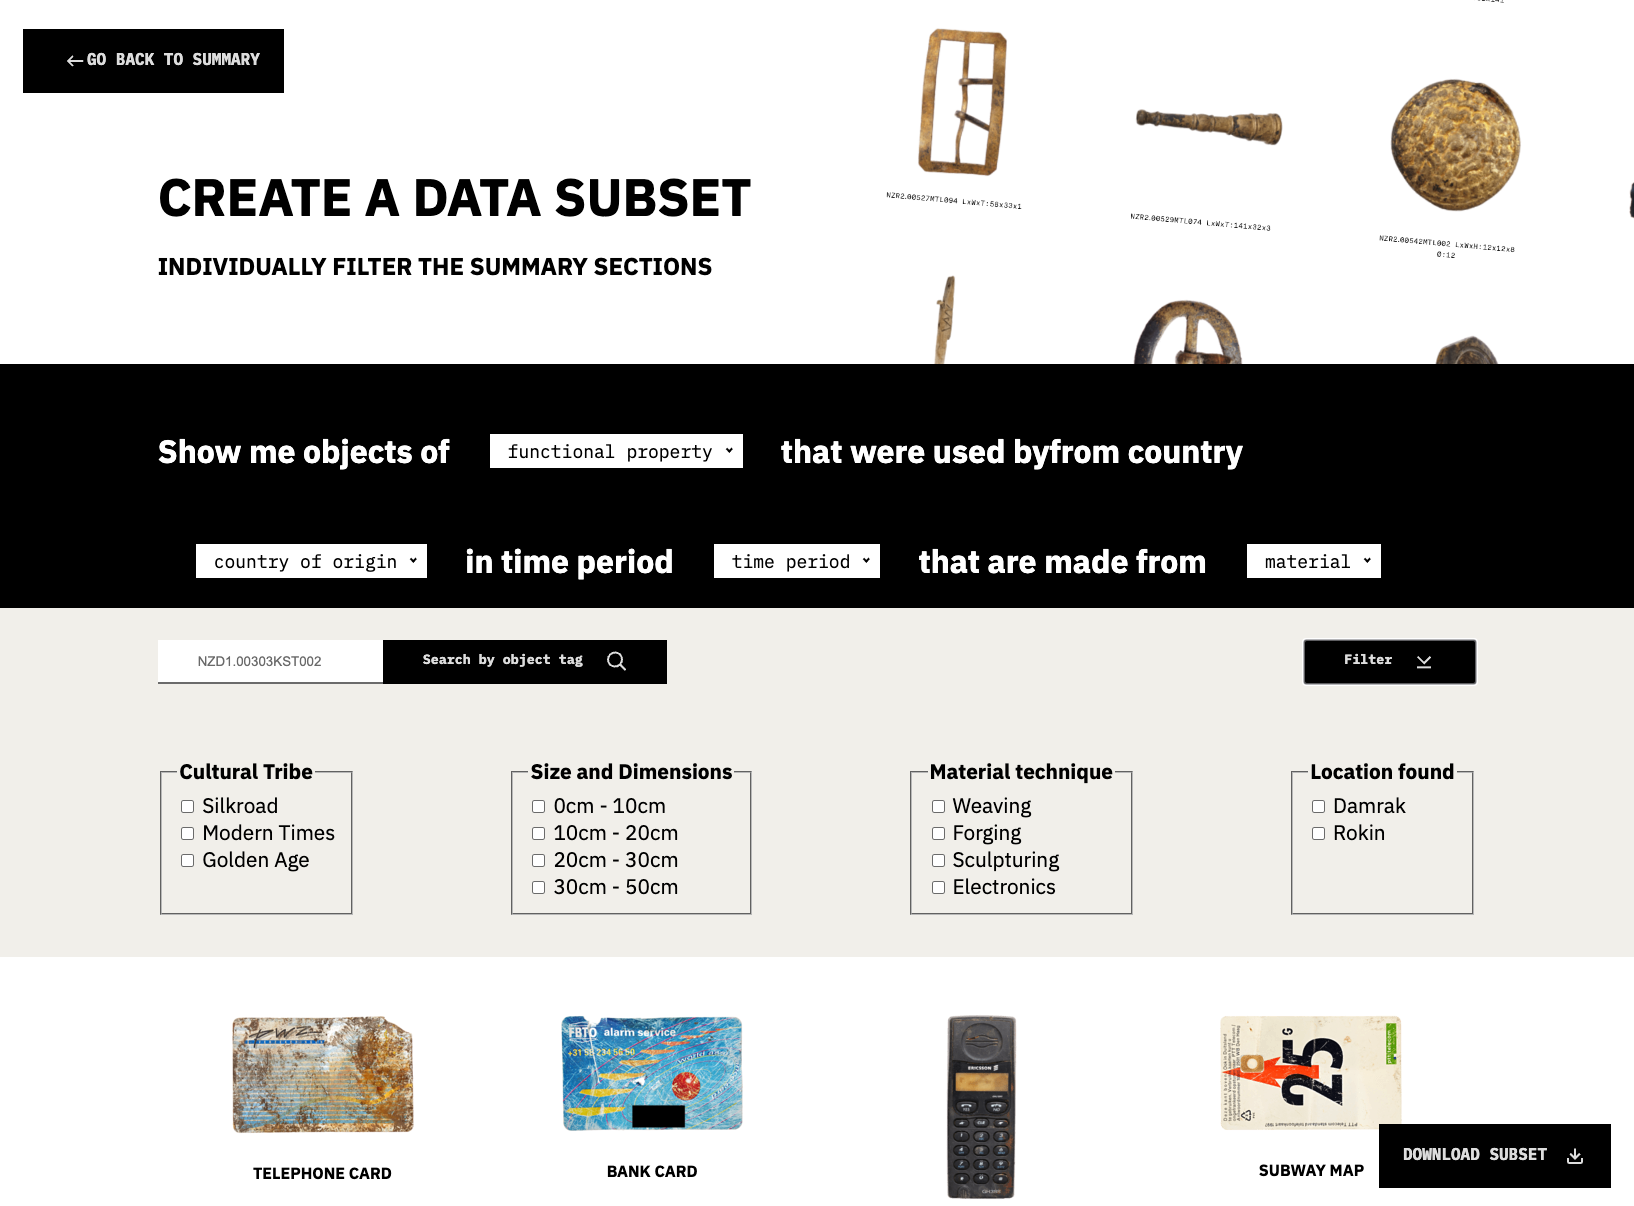
\includegraphics[width=0.6\paperwidth]{website_screenshot-2.png}
    \caption{Screenshot of the detail 'create a subset' page of the website}
    \label{fig:subset}
\end{figure*}
